% http://latexbr.blogspot.com.br/
\documentclass{beamer}
\usepackage[utf8]{inputenc}
\usepackage[T1]{fontenc}
\usepackage[brazil]{babel}
\usepackage{graphics,amssymb,amsfonts,amsmath}
\usepackage{tikz}
\usepackage{tikzsymbols}
\usepackage{enumerate,hyperref}
\usepackage{palatino}	% Fonte sem serifa
\usepackage{ragged2e}	% Paragrafo justificado
\usepackage{minted}	% Highlight para codigos de programacao
\usepackage{booktabs} % tabelas

% Tema, cor e fonte modo matematico
% \usetheme{AnnArbor}
\usetheme{Pittsburgh}
\usecolortheme{orchid}
\usefonttheme[onlymath]{serif}
% Veja mais temas e cores em http://www.hartwork.org/beamer-theme-matrix/

% Colocando numero de paginas no slide
\setbeamertemplate{footline}[frame number]

% Desativando os botoes de navegacao
\beamertemplatenavigationsymbolsempty

% Tela cheia
\hypersetup{pdfpagemode=FullScreen}

% Layout da pagina
\hypersetup{pdfpagelayout=SinglePage}

% Ambiente Bash (minted)
\newminted{bash}{bgcolor=gray!30}

% Titulo
\title{\Huge \LaTeX}
\author{R\'egis da Silva\\ {\texorpdfstring{\color{blue}}{ }about.me/rg3915}}
\institute{\Large {\texorpdfstring{\color{blue}}{ }latexbr.blogspot.com.br}}
\date{}


% **********************************************
\begin{document}
\justifying % Paragrafo justificado

%Neste caso insere somente no primeiro slide.
{%
  \usebackgroundtemplate{%
  \vbox to \paperheight{\vfil\hbox to \paperwidth{\hfil
\includegraphics[width=.5\paperwidth]{img/latex.png}\hfil}\vfil}
  }

  \begin{frame}
  \end{frame}
}

\begin{frame}\frametitle{}
\begin{itemize}
  \item<1-> \Huge O que é?
  \item<2-> \Huge Pra que serve?
  \item<3-> \Huge Como usá-lo?
\end{itemize}
\end{frame}

\begin{frame}\frametitle{}
  \begin{center}
    \Huge No princípio era o homem...
  \end{center}
\end{frame}

% Imagem como plano de fundo
{%
  \usebackgroundtemplate{
    \centering
    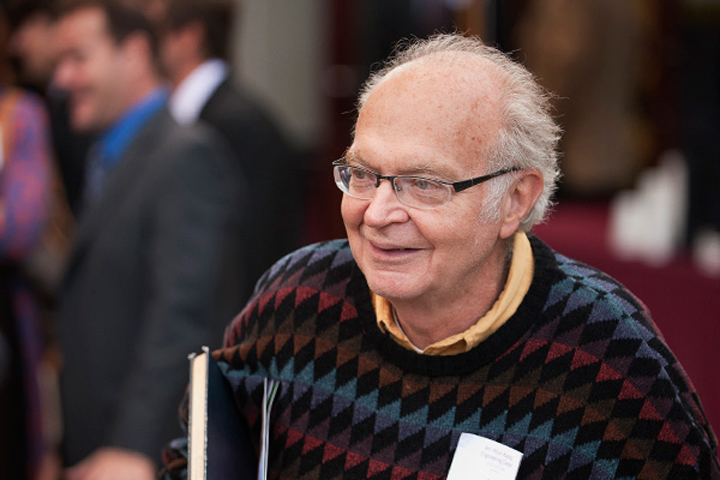
\includegraphics[height=\paperheight]{img/donald_knuth}
  }

  \begin{frame}
    \begin{center}
      \vspace{.7\paperheight}
      \huge \color{white}{E o homem era Donald Knuth.}
    \end{center}
  \end{frame}
}

% Imagem como plano de fundo
{%
  \usebackgroundtemplate{
    \centering
    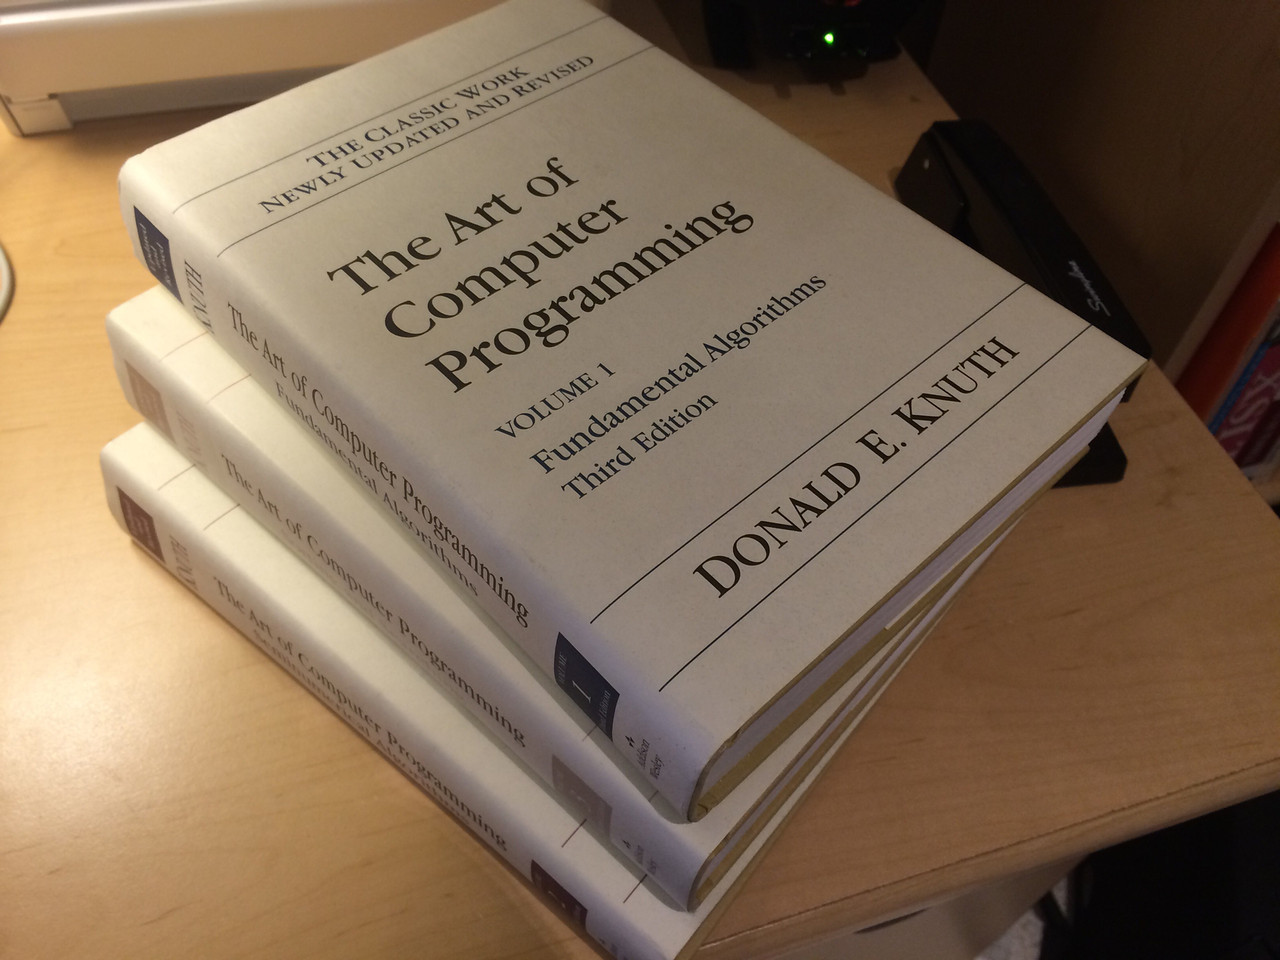
\includegraphics[width=\paperwidth]{img/taocp}
  }

  \begin{frame}
  \end{frame}
}

\begin{frame}\frametitle{}
  \begin{center}
    \Huge Ele criou o \TeX.
  \end{center}
\end{frame}

\begin{frame}\frametitle{}
  \begin{center}
    \Huge Um processador de texto ou sistema de tipografia.
  \end{center}
\end{frame}

\begin{frame}\frametitle{}
  \begin{center}
    \Huge Alguns anos depois...
  \end{center}
\end{frame}

% Imagem como plano de fundo
{%
  \usebackgroundtemplate{
    \centering
    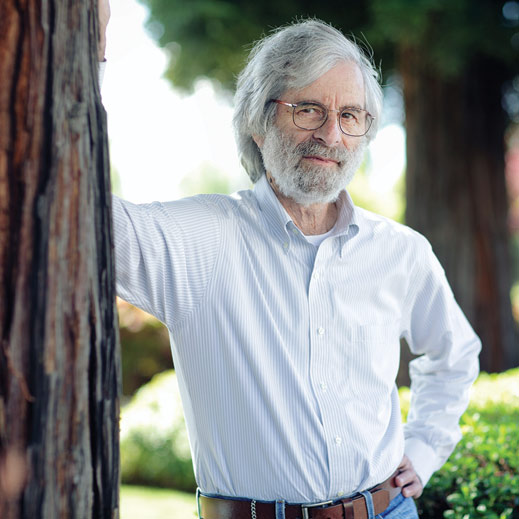
\includegraphics[width=\paperwidth]{img/leslie_lamport}
  }

  \begin{frame}
    \begin{center}
      \vspace{.7\paperheight}
      \Huge \color{blue}{Leslie Lamport}
    \end{center}
  \end{frame}
}

\begin{frame}\frametitle{}
  \begin{center}
    \Huge criou o \LaTeX.
  \end{center}
\end{frame}

\begin{frame}\frametitle{}
  \begin{center}
    \Huge Um conjunto de pacotes \\ de alto nível para o \TeX.
  \end{center}
\end{frame}

\begin{frame}\frametitle{Pra que serve?}
  \begin{center}
    \Large O \LaTeX\ é muito utilizado no meio acadêmico \\ para produção de textos científicos.
  \end{center}
\end{frame}

% Imagem como plano de fundo
{%
  \usebackgroundtemplate{
    \centering
    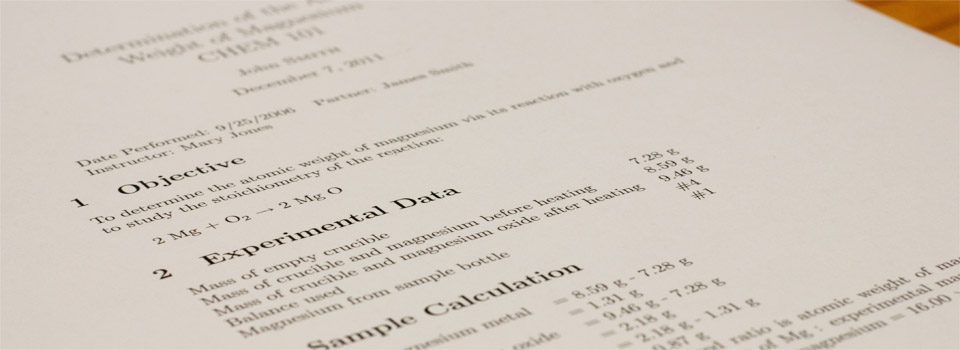
\includegraphics[height=\paperheight]{img/article}
  }

  \begin{frame}\frametitle{Artigos}
  \end{frame}
}

% Imagem como plano de fundo
{%
  \usebackgroundtemplate{
    \centering
    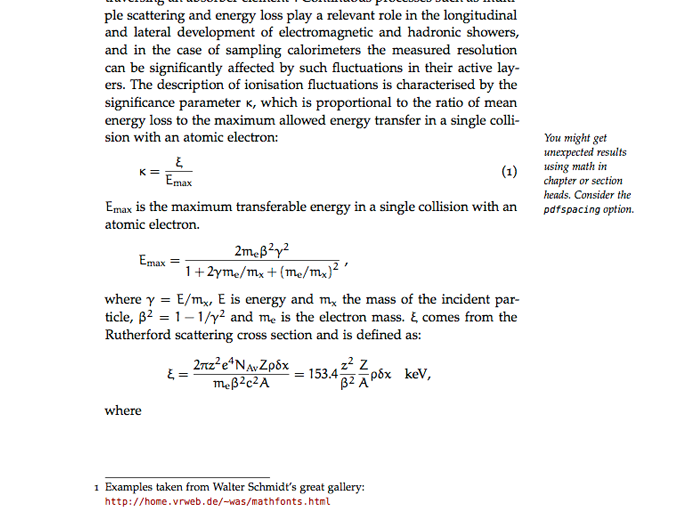
\includegraphics[width=\paperwidth]{img/thesis}
  }

  \begin{frame}\frametitle{Teses}
  \end{frame}
}

% Imagem como plano de fundo
{%
  \usebackgroundtemplate{
    \centering
    
\includegraphics[width=\paperwidth]{img/books}
  }

  \begin{frame}\frametitle{Livros}
  \end{frame}
}

% Imagem como plano de fundo
{%
  \usebackgroundtemplate{
    \centering
    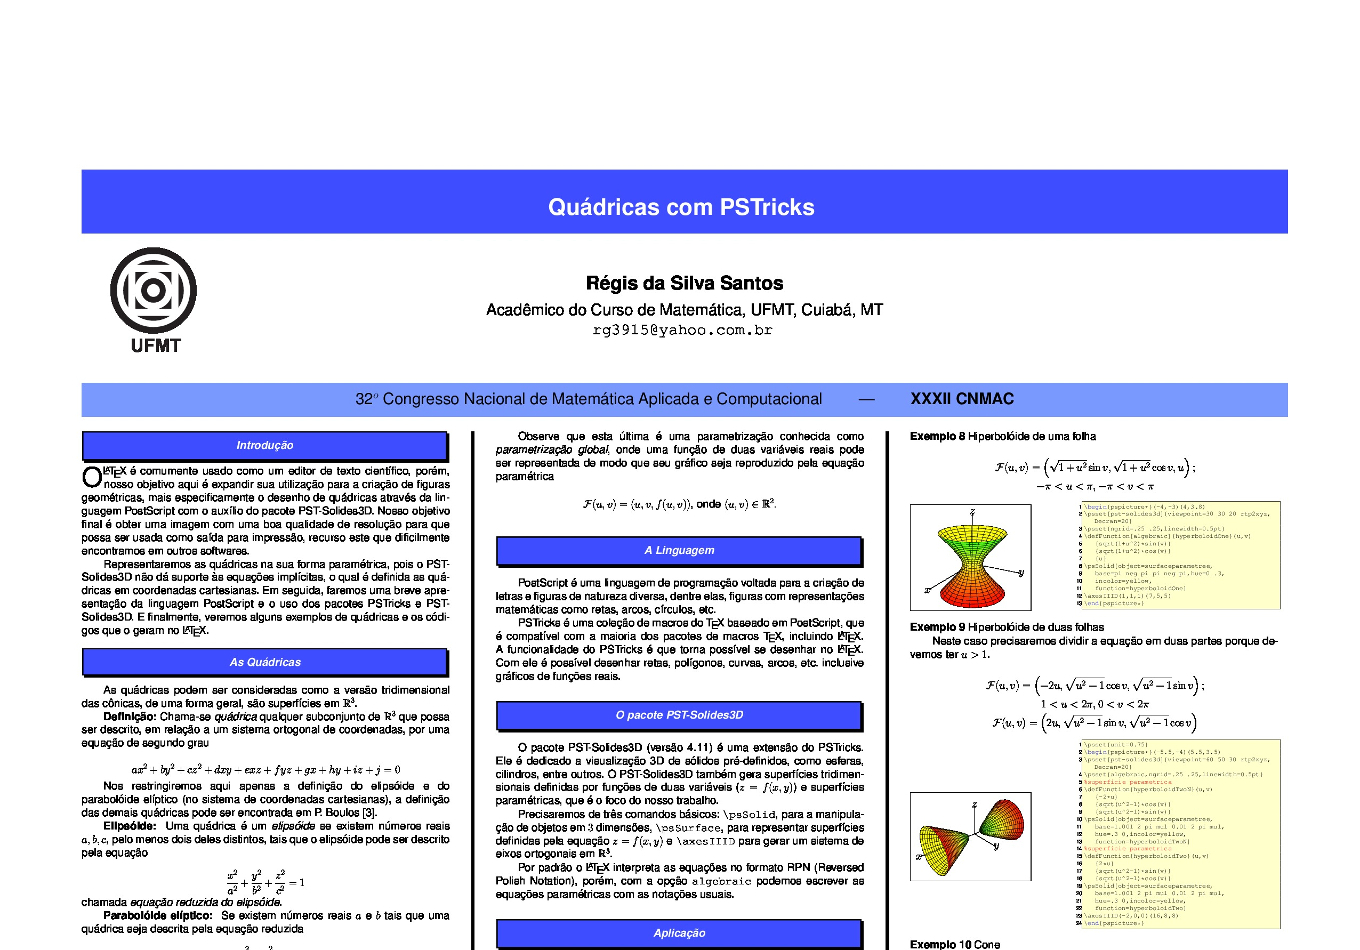
\includegraphics[width=\paperwidth]{img/poster}
  }

  \begin{frame}\frametitle{Posters}
  \end{frame}
}

\begin{frame}\frametitle{Slides}
  \begin{figure}[h]
    \centering
    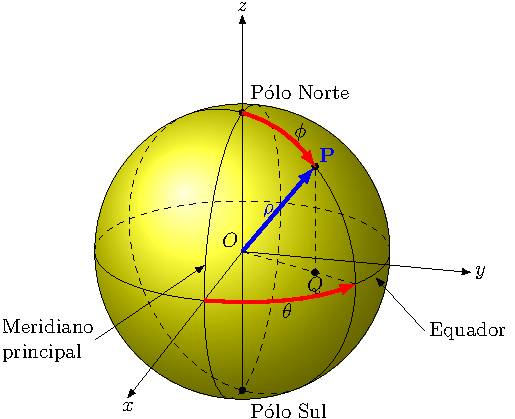
\includegraphics[height=0.6\paperheight]{img/slides}
  \end{figure}
\end{frame}

\begin{frame}\frametitle{Gráficos}
  \begin{figure}[h]
    \centering
    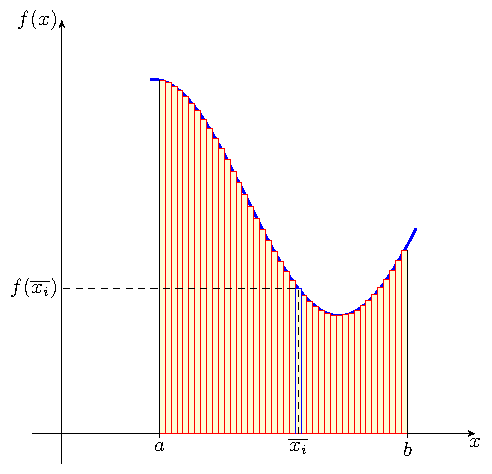
\includegraphics[height=0.6\paperheight]{img/integral}
  \end{figure}
\end{frame}

\begin{frame}\frametitle{Ilustrações Vetoriais}
  \begin{figure}[h]
    \centering
    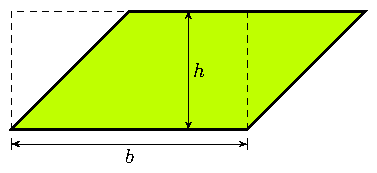
\includegraphics[height=0.4\paperheight]{img/vetorial}
  \end{figure}
\end{frame}

\begin{frame}\frametitle{Expressões Matemáticas}
\[
\int_a^b f(x)dx \equiv (b - a)\frac{f(a) + 4f(\frac{a+b}{2}) + f(b)}{6}
\]
\end{frame}

% Imagem como plano de fundo
{%
  \usebackgroundtemplate{
    \centering
    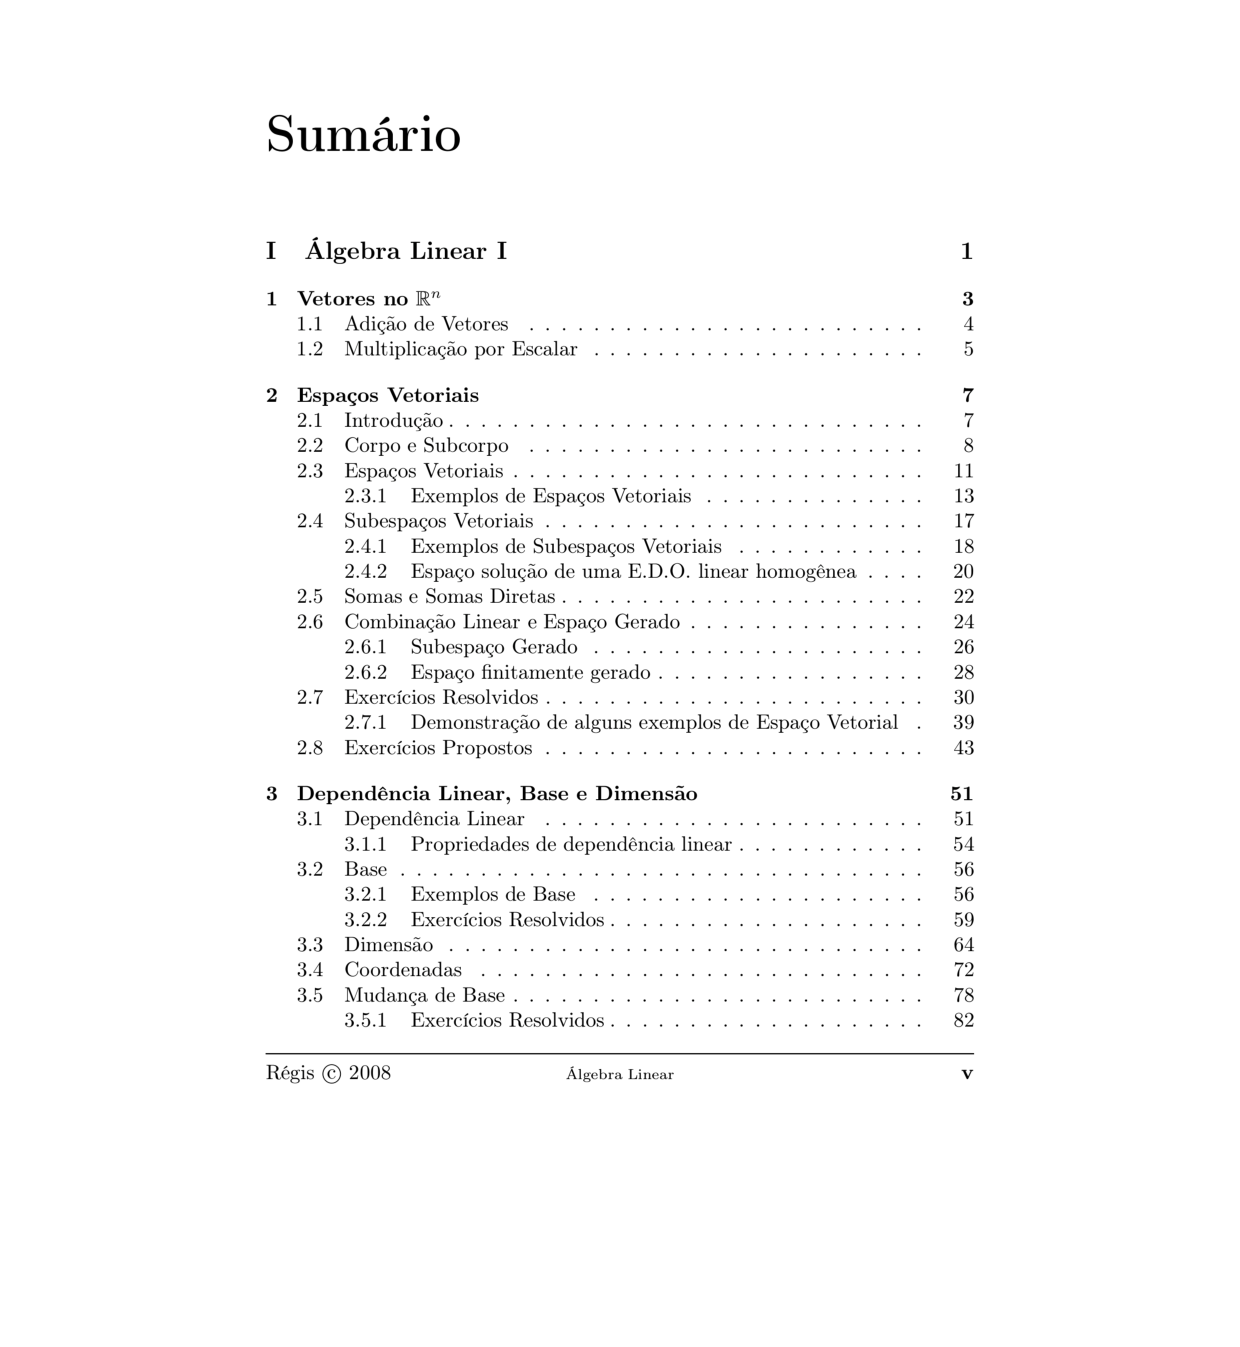
\includegraphics[width=\paperwidth]{img/sumario}
  }

  \begin{frame}
  \end{frame}
}

% Imagem como plano de fundo
{%
  \usebackgroundtemplate{
    \centering
    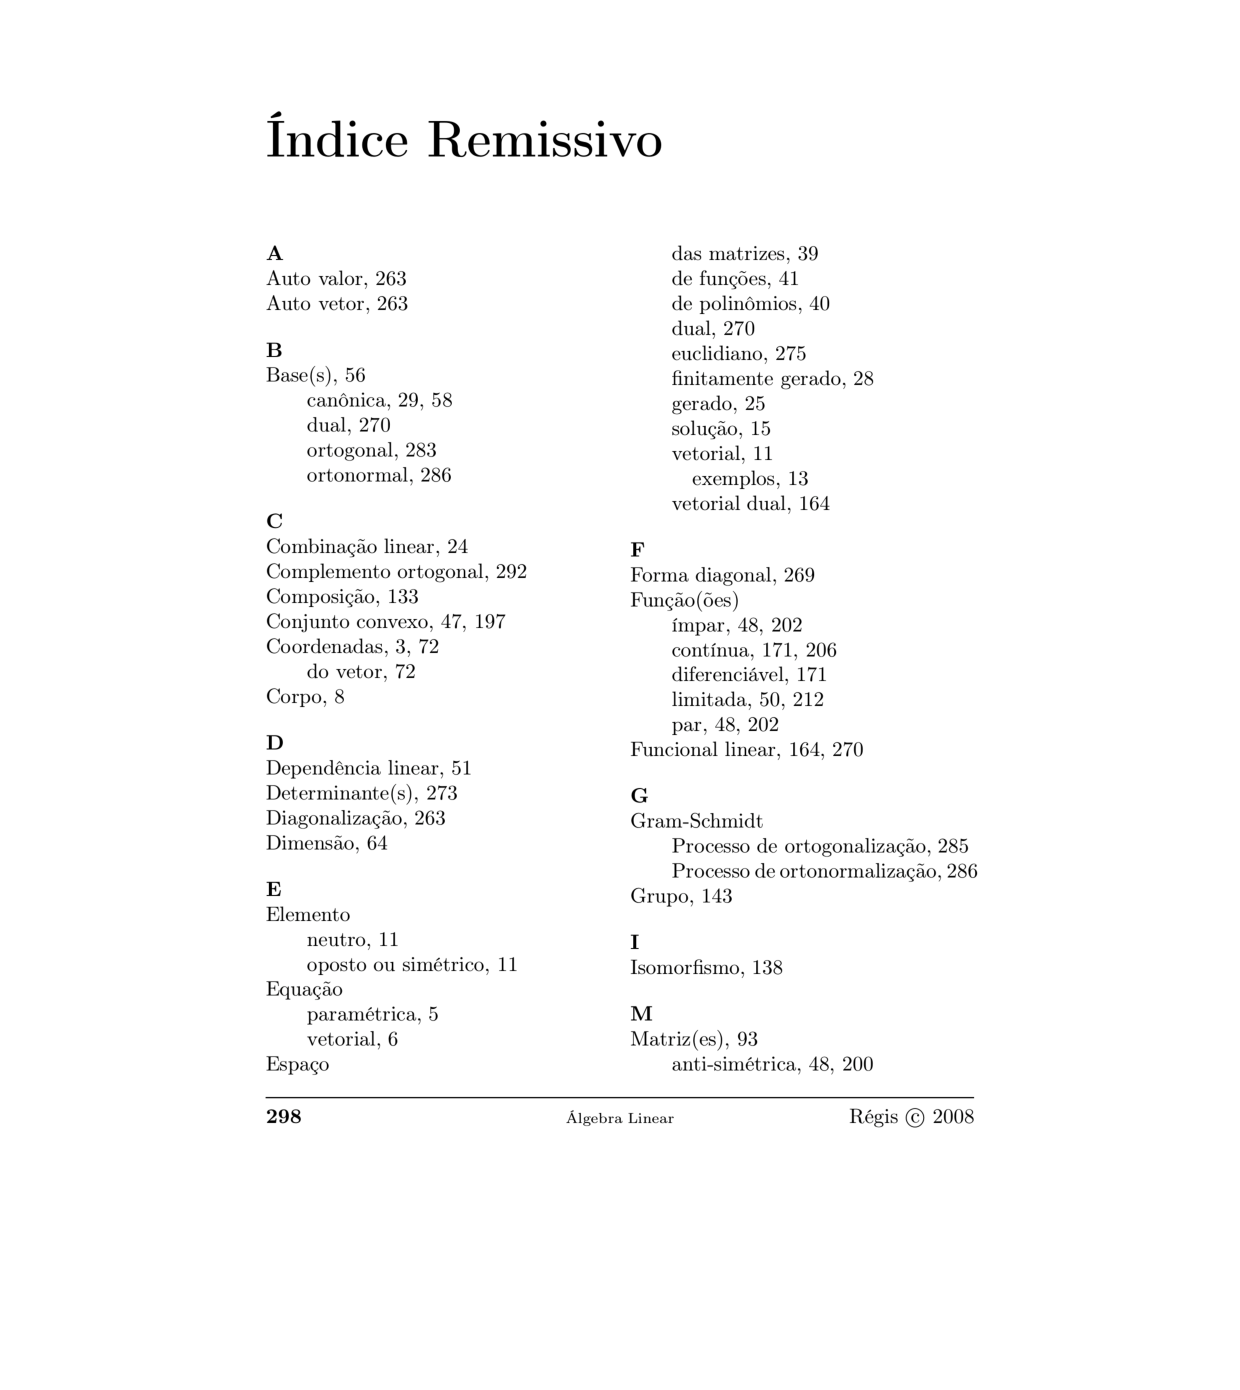
\includegraphics[width=\paperwidth]{img/indice_remissivo}
  }

  \begin{frame}
  \end{frame}
}

\begin{frame}\frametitle{}
  \begin{center}
    \huge Como usar o \LaTeX\ em 3 passos?
  \end{center}
\end{frame}

\begin{frame}[fragile]\frametitle{Edição}
\begin{minted}{latex}
\documentclass[a4paper]{article}
\usepackage[margin=2cm]{geometry}
\usepackage[utf8]{inputenc}
\usepackage[brazil]{babel}
\author{Regis da Silva}
\title{Um Pequeno Artigo}
\date{\today}

\begin{document}
  \maketitle
  Este é o exemplo de um artigo \LaTeX.
\end{document}
\end{minted}
\end{frame}

\begin{frame}[fragile]\frametitle{Compilação}

É o processo que transforma o \tt{meuartigo.tex} em \\ \tt{meuartigo.pdf}

\

\begin{bashcode}
pdflatex meuartigo.tex
\end{bashcode}
\end{frame}

\begin{frame}\frametitle{Visualização}
  \begin{figure}[h]
    \centering
    \fbox{
\includegraphics[width=.7\paperwidth]{examples/meuartigo}}
  \end{figure}
\end{frame}

\begin{frame}\frametitle{}
  \begin{center}
    \huge O \LaTeX\ não é WYSIWYG. \Sadey[1][red]

\

\pause

    \Large Mas existem editores on line com preview em tempo real. \Smiley[1][yellow]
  \end{center}
\end{frame}

\begin{frame}\frametitle{\LaTeX\ on line}
\begin{itemize}
  \item overleaf.com
  \item sharelatex.com
\end{itemize}
\end{frame}

\begin{frame}\frametitle{Instalando \LaTeX}
  \begin{center}
    {\Huge \TeX\ Live 2015} (Win/Linux/Mac)

\

\pause

    {\Huge ou}

\

    {\Huge MiKTeX} (Win)
  \end{center}
\end{frame}

\begin{frame}[fragile]\frametitle{Manuais}

\begin{bashcode}
texdoc latex
\end{bashcode}

\begin{bashcode}
texdoc veryshortguide
\end{bashcode}

\begin{bashcode}
texdoc pgf
\end{bashcode}

\end{frame}

\begin{frame}\frametitle{Manuais}
  \begin{center}
    \Huge IshortBR
  \end{center}
\end{frame}

\begin{frame}\frametitle{Sites}
\begin{itemize}
  \item tug.CTAN
  \item The \TeX\ Catalogue Online
  \item tug.org
  \item Font Catalogue
  \item \TeX ample.net
\end{itemize}
\end{frame}

\begin{frame}\frametitle{Livros}
  \begin{figure}[h]
    \centering
    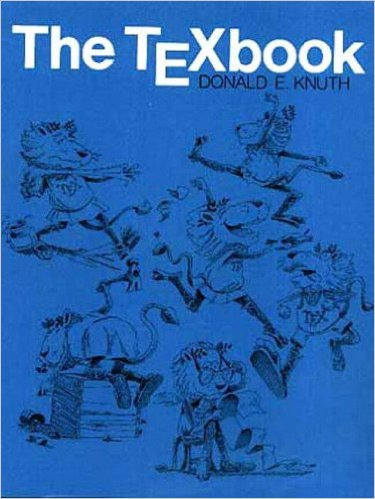
\includegraphics[height=0.6\paperheight]{img/texbook}
    \caption{Donald Knuth. The \TeX book}
  \end{figure}
\end{frame}

\begin{frame}
  \begin{figure}[h]
    \centering
    
\includegraphics[height=0.6\paperheight]{img/latexbook}
    \caption{Leslie Lamport. A Document Preparation System \LaTeX}
  \end{figure}
\end{frame}


\begin{frame}
  \titlepage
\end{frame}

% http://latexbr.blogspot.com.br/

\end{document}
